% presentaciones/sesion06-cap06/sesion06.tex
% Sesión 6 — Capítulo 6: El proceso de decisión de compra
% Laboratorio: Gestión de datos, comportamiento y perfiles del consumidor digital
% Lic. en Mercadotecnia Digital · ESCA Unidad Santo Tomás · IPN
% Fuente de contenido: libro-consumidor-digital/partes/parte2/cap06.tex
% Figuras reutilizadas del libro (TikZ y MATLAB) sin copiarlas: ver \graphicspath y \input.
\documentclass[aspectratio=169,xcolor=dvipsnames]{beamer}
\usetheme{Berlin}

%----------------------------------------------------------------------------------------
%   PALETA INSTITUCIONAL IPN (Manual de Identidad Gráfica, Pantone 222C)
%----------------------------------------------------------------------------------------
\usepackage[dvipsnames,svgnames,x11names]{xcolor}
\definecolor{IPNguinda}{HTML}{6F1D46}       % Pantone 222C oficial — color primario
\definecolor{IPNguindaOsc}{HTML}{45102C}    % sombra / paleta secundaria
\definecolor{IPNguindaClara}{HTML}{F4E9EF}  % fondo de bloques normales
\definecolor{IPNdorado}{HTML}{B8975A}       % dorado — SOLO enlaces y detalles del cierre
\definecolor{IPNterracota}{HTML}{9C5B44}    % alertblock
\definecolor{IPNterracotaClara}{HTML}{F6ECE6}
\definecolor{IPNbronce}{HTML}{8C6B3F}       % exampleblock
\definecolor{IPNbronceClaro}{HTML}{F5F0E3}
\definecolor{IPNgris}{HTML}{58595B}         % texto secundario / notas

% Alias con los nombres de config/colores.tex del libro, para que las figuras
% TikZ del libro se puedan \input sin modificarlas
\colorlet{guindaIPN}{IPNguinda}
\colorlet{guindaIPNOsc}{IPNguindaOsc}
\colorlet{guindaIPNClara}{IPNguindaClara}
\colorlet{doradoIPN}{IPNdorado}
\colorlet{bronceIPN}{IPNbronce}
\colorlet{bronceIPNClaro}{IPNbronceClaro}
\colorlet{grisIPN}{IPNgris}
\colorlet{terracotaIPN}{IPNterracota}
\colorlet{terracotaIPNClara}{IPNterracotaClara}
\definecolor{colorLaboratorio}{HTML}{1B6E7A}

\setbeamercolor{palette primary}{bg=IPNguinda,fg=white}
\setbeamercolor{palette secondary}{bg=IPNguindaOsc,fg=white}
\setbeamercolor{palette tertiary}{bg=IPNguindaOsc,fg=white}
\setbeamercolor{palette quaternary}{bg=IPNguinda,fg=white}
\setbeamercolor{structure}{fg=IPNguinda}
\setbeamercolor{title}{bg=IPNguinda,fg=white}
\setbeamercolor{frametitle}{bg=IPNguinda,fg=white}
\setbeamercolor{block title}{bg=IPNguinda,fg=white}
\setbeamercolor{block body}{bg=IPNguindaClara,fg=black}
\setbeamercolor{block title alerted}{bg=IPNterracota,fg=white}
\setbeamercolor{block body alerted}{bg=IPNterracotaClara,fg=black}
\setbeamercolor{block title example}{bg=IPNbronce,fg=white}
\setbeamercolor{block body example}{bg=IPNbronceClaro,fg=black}
\setbeamercolor{alerted text}{fg=IPNterracota}
\setbeamercolor{item}{fg=IPNguinda}
\setbeamercolor{section in toc}{fg=IPNguinda}
\setbeamercolor{footline}{bg=IPNguindaOsc,fg=white}

\usepackage[spanish,es-noshorthands,es-nodecimaldot]{babel}
\usepackage{csquotes}
\usepackage{hyperref}
\usepackage{graphicx}
\usepackage{booktabs}
\usepackage{array}
\usepackage{amsmath}
\setbeamertemplate{caption}[numbered]
\usepackage{xurl}
\usepackage{adjustbox}
\usepackage{tikz}
\usetikzlibrary{arrows.meta,positioning}
\usepackage{pgfplots}
\pgfplotsset{compat=1.18}

\graphicspath{{Figures/}{../../libro-consumidor-digital/figuras/matlab/}}
\newcommand{\figtikz}[1]{../../libro-consumidor-digital/figuras/tikz/#1}
\newcommand{\fuente}[1]{{\tiny\color{IPNgris}Fuente: #1}}

\hypersetup{
    colorlinks=true,
    linkcolor=IPNdorado,
    filecolor=IPNguinda,
    urlcolor=IPNguinda,
    citecolor=IPNguinda,
    pdftitle={Sesion 6 - El proceso de decision de compra},
    pdfauthor={Dr. Aboud Barsekh-Onji},
}

%----------------------------------------------------------------------------------------
%   CODE LISTINGS — sintaxis ESTÁNDAR del lenguaje
%----------------------------------------------------------------------------------------
\usepackage{listings}
\definecolor{backcolour}{rgb}{0.97,0.97,0.99}
\definecolor{codegreen}{rgb}{0,0.6,0}

\lstdefinestyle{MATLABStyle}{
  language=Matlab,
  basicstyle=\ttfamily\scriptsize,
  keywordstyle=\color{blue}\bfseries,
  commentstyle=\color{codegreen},
  stringstyle=\color{violet},
  breaklines=true,
  numbers=left,
  numbersep=5pt,
  frame=lines,
  backgroundcolor=\color{backcolour}
}
\lstset{style=MATLABStyle}

%----------------------------------------------------------------------------------------
%   TITLE CONFIGURATION
%----------------------------------------------------------------------------------------
\logo{
\includegraphics[height=0.75cm]{ipn-escudo.png}}
\title[Sesión 6 · El proceso de decisión]{El proceso de decisión de compra}
\subtitle{Sesión 6 · Unidad II — Capítulo 6}
\author{Dr. Aboud Barsekh-Onji}
\institute[IPN]{
    Instituto Politécnico Nacional \\
    \small ESCA Unidad Santo Tomás · Lic. en Mercadotecnia Digital \\
    \footnotesize Laboratorio: Gestión de datos, comportamiento y perfiles del consumidor digital
}
\date{\today}

%----------------------------------------------------------------------------------------
%   AUTO AGENDA AT EACH SECTION
%----------------------------------------------------------------------------------------
\AtBeginSection[]{
  \begin{frame}{Agenda}
    \tableofcontents[currentsection]
  \end{frame}
}



\begin{document}

\begin{frame}
    \titlepage
    \vspace{-4pt}
    \begin{center}
        {\tiny\color{IPNgris} ORCID: \href{https://orcid.org/0009-0004-5440-8092}{0009-0004-5440-8092}}
    \end{center}
\end{frame}

%------------------------------------------------
\section{Encuadre}
%------------------------------------------------

\begin{frame}{Ficha de la sesión}
\begin{columns}[T]
  \column{0.52\textwidth}
  \begin{block}{Unidad II}
    \small Proceso de toma de decisión de compra digital
  \end{block}
  \begin{block}{Tema del programa (2.1 Proceso de toma de decisiones de compra)}
    \scriptsize
    \begin{itemize}
      \item[2.1.1] Reconocimiento de necesidades y/o deseos
      \item[2.1.2] Búsqueda de información
      \item[2.1.3] Evaluación de alternativas
      \item[2.1.4] Decisión de compra-consumo
      \item[2.1.5] Evaluación post-compra-satisfacción
    \end{itemize}
  \end{block}
  \column{0.44\textwidth}
  \begin{block}{Carga horaria}
    \small Teoría 3.0 h · Práctica 2.0 h\\ Aprendizaje autónomo 1.0 h
  \end{block}
  \begin{exampleblock}{Competencia de la unidad}
    \small Examina el proceso de toma de decisiones de compra del consumidor digital a partir de su recorrido y figuras participantes.
  \end{exampleblock}
\end{columns}
\end{frame}

\begin{frame}{Al terminar la sesión podrás\ldots}
\begin{enumerate}
  \item \textbf{Describir} las cinco etapas del proceso de decisión y qué cambia en cada una en el entorno digital.
  \vspace{4pt}
  \item \textbf{Diferenciar} una regla compensatoria de una no compensatoria y predecir cuándo elegirán distinto.
  \vspace{4pt}
  \item \textbf{Distinguir} un \textit{nudge} de un patrón oscuro con un criterio verificable.
  \vspace{4pt}
  \item \textbf{Aplicar} tres reglas de decisión a las mismas alternativas y localizar el peso en que cambia la elección.
\end{enumerate}
\vspace{6pt}
\begin{alertblock}{Recordatorio}
  Aprendizaje autónomo de la sesión anterior (Google Analytics 4): entrega en la fecha acordada en clase, en su carpeta del portafolio.
\end{alertblock}
\end{frame}

\begin{frame}{Arranque: la última compra que no planeabas}
\begin{columns}[T]
  \column{0.55\textwidth}
  \begin{exampleblock}{Pregunta de arranque}
    Piensen en una compra en línea \textbf{que no tenían planeada}.\\[4pt]
    ¿Qué la disparó: una necesidad, una notificación, un anuncio, un amigo? ¿Cuántas alternativas compararon antes de pagar?
  \end{exampleblock}
  \vspace{4pt}
  {\small\color{IPNgris} Puente con la Unidad I: cada paso de esa compra dejó un dato.}
  \column{0.41\textwidth}
  \begin{block}{Dinámica (10 min)}
    \small
    \begin{enumerate}
      \item Individual: anoten qué la disparó (2 min).
      \item Parejas: ¿qué etapas reconocen? ¿cuál fue más corta?
      \item Pizarrón: cuántos fueron disparados \textbf{por el canal} y no por una carencia.
    \end{enumerate}
  \end{block}
\end{columns}
\end{frame}

%------------------------------------------------
\section[Apertura]{Caso de apertura}
%------------------------------------------------

\begin{frame}{Mariana y los audífonos (caso ficticio)}
\begin{exampleblock}{Caso ilustrativo (ficticio)}
  A las once de la noche, Mariana recibe: \enquote{\textbf{Quedan 2 piezas. Tu carrito expira en 10 minutos}}. No había abierto la aplicación en toda la semana. \textbf{Compra.}
\end{exampleblock}
\begin{alertblock}{A la mañana siguiente}
  El modelo que eligió tarda \textbf{siete días} en llegar. Otro, de precio similar, llegaba en \textbf{dos}.
\end{alertblock}
\vspace{4pt}
\begin{block}{Tres preguntas}
  \small ¿Mariana \emph{reconoció} una necesidad o se la fabricaron? ¿Evaluó alternativas o reaccionó a un temporizador? ¿Qué parte de la decisión fue suya?
\end{block}
\end{frame}

%------------------------------------------------
\section[Proceso]{2.1 El proceso de decisión}
%------------------------------------------------

\begin{frame}{Cinco etapas y dos variantes digitales}
\begin{center}
  \adjustbox{max width=0.97\linewidth,max height=0.52\textheight}{\input{\figtikz{cap06-proceso-decision}}}
\end{center}
\vspace{2pt}
\begin{itemize}
  \scriptsize
  \item Esquema de los tres textos de la bibliografía oficial (Solomon y Russell, 2023; Hoyer et al., 2024; Kotler et al., 2021).
  \item En internet el orden se tuerce: el algoritmo dispara la 1, el temporizador comprime la 3 y la reseña propia es la 2 de otro.
\end{itemize}
\fuente{elaboración propia.}
\end{frame}

\begin{frame}{2.1.1 Reconocimiento: de la brecha al disparador}
\begin{columns}[T]
  \column{0.48\textwidth}
  \begin{block}{Modelo clásico}
    \small Hay una \textbf{brecha} entre el estado actual y el deseado. Nace \textbf{en la persona}: se acabó el café, quiero otro teléfono.
  \end{block}
  \column{0.48\textwidth}
  \begin{alertblock}{Reconocimiento inducido}
    \small Notificación, recomendación algorítmica o \textit{retargeting} generan necesidad percibida \textbf{sin carencia previa}. Nace \textbf{en el diseño del canal}.
  \end{alertblock}
\end{columns}
\vspace{6pt}
\begin{center}\small No es ilegítimo recordar. Lo que cambia es la pregunta: \textbf{¿quién decidió que había una brecha?}\end{center}
\end{frame}

\begin{frame}{2.1.2 Búsqueda: tres tipos de fuente que se cruzan}
\begin{columns}[T]
  \column{0.31\textwidth}
  \begin{block}{De la marca}
    \small Sitio propio, correo, catálogo.
  \end{block}
  \column{0.31\textwidth}
  \begin{exampleblock}{De terceros}
    \small Buscadores, comparadores, reseñas.
  \end{exampleblock}
  \column{0.31\textwidth}
  \begin{block}{Sociales}
    \small Recomendaciones de pares, contenido de usuarios.
  \end{block}
\end{columns}
\vspace{6pt}
\begin{alertblock}{Webrooming y showrooming}
  \small \textbf{Webrooming:} investigar en línea y comprar en tienda. \textbf{Showrooming:} probar en tienda y comprar en línea. Coexisten y dependen de la \textbf{categoría de producto}, no de un tipo fijo de consumidor (Halibas et al., 2023).
\end{alertblock}
\end{frame}

\begin{frame}{2.1.3 Evaluación: casi nadie pondera todo}
\begin{columns}[T]
  \column{0.50\textwidth}
  \begin{block}{Racionalidad limitada}
    \small Con tiempo y atención limitados se busca una opción \textbf{suficientemente buena}, no la óptima (Simon, 1955).
  \end{block}
  \begin{exampleblock}{Estrategias adaptativas}
    \small Ante \textbf{muchas} alternativas se descarta primero y se compara después (Payne et al., 1988).
  \end{exampleblock}
  \column{0.46\textwidth}
  \begin{alertblock}{Heurísticas}
    \small Atajos de juicio con información abundante o incierta: \textbf{representatividad, disponibilidad y anclaje} (Tversky y Kahneman, 1974).\\[3pt]
    La interfaz puede \textbf{activarlas o mitigarlas}.
  \end{alertblock}
\end{columns}
\end{frame}

\begin{frame}{Tres reglas, dos familias}
\begin{columns}[c]
  \column{0.52\textwidth}
  \begin{center}
    \resizebox{\linewidth}{!}{\input{\figtikz{cap06-reglas-decision}}}
  \end{center}
  \column{0.44\textwidth}
  \footnotesize
  \begin{tabular}{@{}>{\raggedright}p{1.9cm}>{\raggedright\arraybackslash}p{3.6cm}@{}}
    \toprule
    \textbf{Regla} & \textbf{Cómo decide} \\
    \midrule
    Aditiva & Suma puntaje $\times$ peso. Lo bueno compensa lo malo. \\
    Conjuntiva & Mínimo por atributo; falla en uno y queda fuera. \\
    Lexicográfica & Manda el atributo más importante; el siguiente solo desempata. \\
    \bottomrule
  \end{tabular}
\end{columns}
\fuente{elaboración propia con base en Payne et al. (1988).}
\end{frame}

\begin{frame}{Frontera: del nudge al patrón oscuro}
\begin{center}
  \resizebox{0.62\linewidth}{!}{\input{\figtikz{cap06-nudge-dark}}}
\end{center}
\vspace{2pt}
\begin{itemize}
  \scriptsize
  \item \textbf{Nudge} (Thaler y Sunstein, 2008): modifica el contexto de decisión \textbf{sin prohibir opciones} ni cambiar incentivos de forma significativa.
  \item Una tienda en línea \textbf{es} una arquitectura de elección: orden, insignias, temporizadores, pago en un clic.
  \item Mathur et al. (2019) rastrearon 11\,000 sitios: las mismas palancas se usan para acelerar la decisión y reducir la comparación real.
\end{itemize}
\fuente{elaboración propia a partir de Thaler y Sunstein (2008) y Mathur et al. (2019).}
\end{frame}

\begin{frame}{El criterio: información veraz y salida fácil}
\footnotesize
\begin{center}
\begin{tabular}{@{}>{\raggedright}p{1.7cm}>{\raggedright}p{4.4cm}>{\raggedright\arraybackslash}p{4.8cm}@{}}
\toprule
\textbf{Palanca} & \textbf{Nudge} & \textbf{Patrón oscuro} \\
\midrule
Escasez & Muestra el inventario real cuando queda poco. & Anuncia \enquote{quedan 2} con un número fijo. \\
Urgencia & Informa la fecha real en que termina la promoción. & Temporizador que se reinicia al recargar. \\
Prueba social & Calificación promedio con el total de reseñas. & \enquote{Alguien compró esto} generado al azar. \\
Salida & Cancelar cuesta lo mismo que contratar. & Contratar, un clic; cancelar, llamar por teléfono. \\
\bottomrule
\end{tabular}
\end{center}
\vspace{2pt}
\begin{alertblock}{Dato experimental}
  \scriptsize Luguri y Strahilevitz (2021): los patrones leves \textbf{más que duplicaron} la probabilidad de conservar un servicio no pedido; los agresivos, \textbf{casi la cuadruplicaron}.
\end{alertblock}
\fuente{elaboración propia; ejemplos ilustrativos.}
\end{frame}

\begin{frame}{2.1.4 y 2.1.5: pagar no es consumir, y la reseña cierra el bucle}
\begin{columns}[T]
  \column{0.48\textwidth}
  \begin{block}{Decisión de compra-consumo}
    \small Pesa la \textbf{fricción} del pago: pasos del \textit{checkout}, medios de pago, cuándo aparece el envío. \textbf{Comprar} es transferir el pago; \textbf{consumir}, usar. La satisfacción depende de lo segundo.
  \end{block}
  \column{0.48\textwidth}
  \begin{exampleblock}{Post-compra}
    \small Se compara la experiencia con la expectativa. En digital se vuelve \textbf{pública}: calificación, reseña, \textit{unboxing}. Alimenta la etapa 2 de \textbf{otros}. El proceso es un \textbf{bucle}, no una línea.
  \end{exampleblock}
\end{columns}
\vspace{6pt}
{\small\color{IPNgris} Court et al. (2009) documentaron el retroceso a evaluar hace más de quince años. Lo vemos en la próxima sesión.}
\end{frame}

%------------------------------------------------
\section[Evidencia]{Evidencia: México}
%------------------------------------------------

\begin{frame}{Dimensión del comercio digital en México (2025)}
\footnotesize
\begin{center}
\begin{tabular}{@{}>{\raggedright}p{5.4cm}>{\raggedright}p{2.5cm}>{\raggedright\arraybackslash}p{3.8cm}@{}}
\toprule
\textbf{Indicador} & \textbf{Cifra} & \textbf{Fuente} \\
\midrule
Población de 6 años o más usuaria de internet & 86.1\,\% & ENDUTIH 2025 (INEGI) \\
Personas usuarias que compraron en línea & 37.3\,\% & ENDUTIH 2025 (INEGI) \\
Comercio electrónico minorista & 941 mil millones de pesos & AMVO, Estudio de Venta Online 2026 \\
Participación en ventas minoristas & 17.7\,\% & AMVO 2026 \\
Compradores digitales & 77.2 millones & AMVO 2026 \\
\bottomrule
\end{tabular}
\end{center}
\vspace{2pt}
\begin{alertblock}{Lectura cuidadosa}
  \scriptsize Que 37.3\,\% haya comprado en línea \textbf{no} significa que 62.7\,\% decida fuera de internet: puede haber investigado en línea y pagado en tienda (\textit{webrooming}). Las dos fuentes miden cosas distintas: no se suman.
\end{alertblock}
\fuente{INEGI (2026); Asociación Mexicana de Venta Online (2026).}
\end{frame}

%------------------------------------------------
\section[Laboratorio]{Laboratorio MATLAB}
%------------------------------------------------

\begin{frame}{Laboratorio: tres reglas sobre las mismas alternativas}
\begin{block}{Objetivo}
  Aplicar la regla aditiva, la conjuntiva y la lexicográfica a seis alternativas \textbf{ficticias}, comparar la elección de cada una y localizar el peso del precio donde cambia la decisión.
\end{block}
\begin{columns}[T]
  \column{0.52\textwidth}
  \begin{exampleblock}{Normalización 0--10 (min-max)}
    \scriptsize
    \[ s_{ij} = 10\,\frac{x_{ij}-\min_i x_{ij}}{\max_i x_{ij}-\min_i x_{ij}} \]
    En precio y entrega (costo): $s_{ij}\leftarrow 10-s_{ij}$. Así 10 siempre es \enquote{lo mejor}.
  \end{exampleblock}
  \column{0.44\textwidth}
  \begin{block}{Utilidad aditiva}
    \scriptsize
    \[ U_i=\sum_j w_j\,s_{ij},\qquad \sum_j w_j=1 \]
    Conjuntiva: $s_{ij}\ge u$ en \textbf{todos} los $j$. Lexicográfica: tolerancia $\tau$.
  \end{block}
\end{columns}
\end{frame}

\begin{frame}[fragile]{El script: \texttt{cap06\_alternativas.m}}
\begin{columns}[T]
  \column{0.62\textwidth}
\begin{lstlisting}[basicstyle=\ttfamily\tiny]
%% ==================================
%  PARAMETROS: UNICA SECCION QUE
%  EL ESTUDIANTE DEBE EDITAR
%  ==================================
pesoPrecio = 0.40;
pesoCalidad = 0.30;
pesoEntrega = 0.15;
pesoResenas = 0.15;
umbralMinimo = 3.5;      % conjuntiva
atributoPrioritario = 2; % 1 precio,
  % 2 calidad, 3 entrega, 4 resenas
toleranciaLex = 0.5;     % lexicografica
\end{lstlisting}
  \column{0.34\textwidth}
  \begin{block}{Reglas y rangos}
    \scriptsize
    \begin{itemize}
      \item Pesos: reales $\geq 0$, al menos uno $>0$; el script los normaliza.
      \item Umbral y tolerancia: entre 0 y 10.
      \item Datos \textbf{sintéticos} y marcas ficticias; no hay azar.
    \end{itemize}
  \end{block}
  \begin{exampleblock}{Sin MATLAB}
    \scriptsize \texttt{cap06\_alternativas\_\allowbreak interactivo.html}: mismos parámetros y casos A, B, C.
  \end{exampleblock}
\end{columns}
\end{frame}

\begin{frame}{Salida: utilidad y elección de cada regla}
\begin{center}
  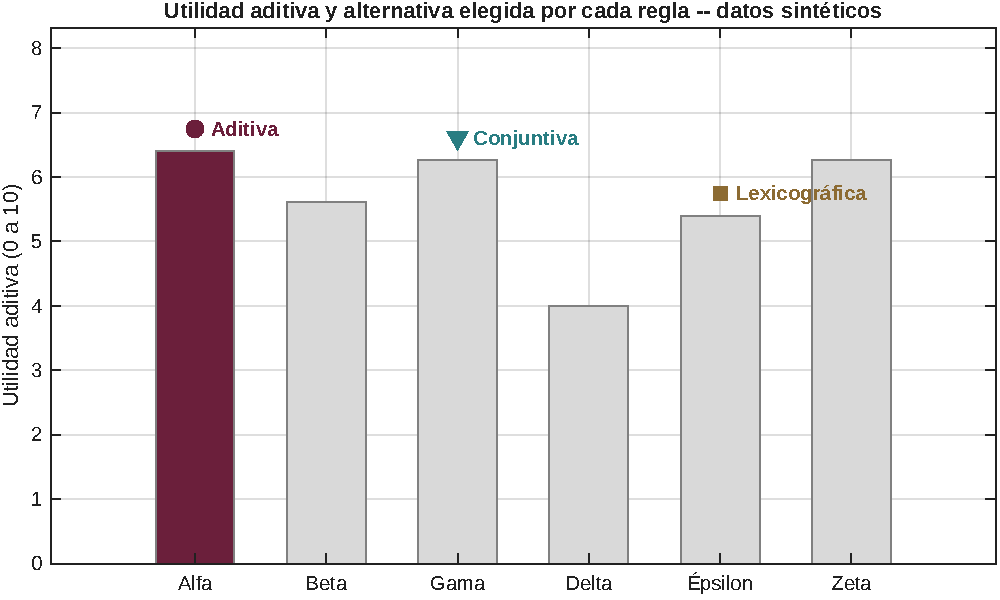
\includegraphics[width=\linewidth,height=0.62\textheight,keepaspectratio]{cap06_reglas_decision.pdf}
\end{center}
\vspace{-4pt}
\begin{center}
  \small Con los valores por defecto: aditiva $\to$ \textbf{Alfa} · conjuntiva $\to$ \textbf{Gama} · lexicográfica $\to$ \textbf{Épsilon}
\end{center}
\fuente{elaboración propia, MATLAB, datos sintéticos.}
\end{frame}

\begin{frame}{Interpretación de negocio}
\begin{columns}[c]
  \column{0.48\textwidth}
  \begin{block}{Tres preguntas distintas}
    \small \textbf{Aditiva:} ¿qué rinde más en promedio? \textbf{Conjuntiva:} ¿cuál no tiene un defecto inaceptable? \textbf{Lexicográfica:} ¿cuál es mejor en lo único que importa?
  \end{block}
  \begin{alertblock}{El error costoso}
    \small Diseñar la ficha de producto para \textbf{una} regla y perder a quienes deciden con otra.
  \end{alertblock}
  \column{0.48\textwidth}
  \begin{exampleblock}{Ninguna está equivocada}
    \small La regla de decisión \textbf{cambia el producto elegido} con los mismos datos. Por eso importa saber qué regla usa tu cliente.
  \end{exampleblock}
\end{columns}
\end{frame}

\begin{frame}{Salida: ¿cuándo cambia la elección?}
\begin{center}
  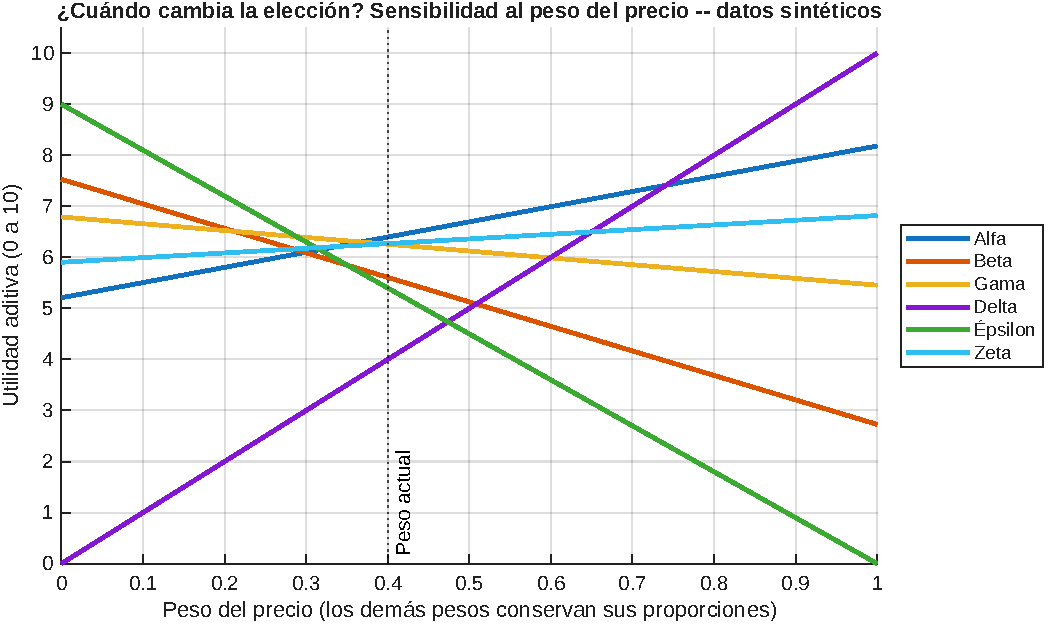
\includegraphics[width=\linewidth,height=0.62\textheight,keepaspectratio]{cap06_sensibilidad_peso.pdf}
\end{center}
\vspace{-4pt}
\begin{center}
  \small Al barrer el peso del precio de 0 a 1, la regla aditiva cambia de ganador \textbf{tres veces}.
\end{center}
\fuente{elaboración propia, MATLAB, datos sintéticos.}
\end{frame}

\begin{frame}{Ejercicio propuesto: tres corridas}
\begin{columns}[T]
  \column{0.52\textwidth}
  \begin{exampleblock}{Casos (solo el bloque de parámetros)}
    \scriptsize
    \begin{itemize}
      \item[\textbf{A}] Valores por defecto.
      \item[\textbf{B}] \textbf{El precio domina}: pesos 0.80 / 0.10 / 0.05 / 0.05.
      \item[\textbf{C}] \textbf{Mínimo exigente}: pesos por defecto, \texttt{umbralMinimo} = 6 y \texttt{atributoPrioritario} = 3.
    \end{itemize}
  \end{exampleblock}
  \column{0.44\textwidth}
  \footnotesize
  \begin{tabular}{@{}lccc@{}}
    \toprule
    Caso & Aditiva & Conjunt. & Lexic. \\
    \midrule
    A & \rule{0.9cm}{0.4pt} & \rule{0.9cm}{0.4pt} & \rule{0.9cm}{0.4pt} \\[2pt]
    B & \rule{0.9cm}{0.4pt} & \rule{0.9cm}{0.4pt} & \rule{0.9cm}{0.4pt} \\[2pt]
    C & \rule{0.9cm}{0.4pt} & \rule{0.9cm}{0.4pt} & \rule{0.9cm}{0.4pt} \\
    \bottomrule
  \end{tabular}
\end{columns}
\vspace{2pt}
\begin{block}{Respondan con sus corridas}
  \scriptsize
  \begin{enumerate}
    \item Caso B: ¿qué elige la aditiva y por qué la conjuntiva no la acepta?
    \item Caso C: ¿qué pasa con la conjuntiva y qué debería hacer el consumidor?
    \item ¿Cuándo conviene \textbf{descartar} con una regla no compensatoria y \textbf{elegir} con una compensatoria? Relaciónenlo con Payne et al. (1988).
  \end{enumerate}
\end{block}
\end{frame}

\begin{frame}{Primer insumo de la práctica «Recorrido del consumidor digital»}
\begin{columns}[T]
  \column{0.54\textwidth}
  \begin{block}{Una práctica, cuatro sesiones}
    \small La Unidad II tiene \textbf{una sola práctica de 15 h} con un entregable único. Crece capítulo a capítulo sobre \textbf{un caso real} de compra digital que cada equipo elige hoy.
  \end{block}
  \column{0.42\textwidth}
  \begin{exampleblock}{Hoy producen}
    \scriptsize
    \begin{itemize}
      \item El caso elegido (propio o de una persona entrevistada).
      \item Las cinco etapas de ese caso: qué ocurrió y qué \textbf{canal} intervino.
      \item ¿Hubo reconocimiento inducido?
    \end{itemize}
  \end{exampleblock}
\end{columns}
\end{frame}

\begin{frame}{Práctica con sus propios datos: app HTML}
\begin{columns}[T]
  \column{0.54\textwidth}
  \begin{block}{\texttt{cap06\_alternativas\_datos\_propios.html}}
    \small Sin MATLAB y sin conexión: suban un Excel con \textbf{sus datos} y recorran 5 pasos:
    \scriptsize
    \begin{enumerate}
      \item Calidad de los datos y escala común 0 a 10.
      \item Regla aditiva y alternativa elegida.
      \item Reglas conjuntiva y lexicográfica.
      \item Barrido: ¿qué tan frágil es la elección?
      \item Lectura de negocio y descarga en Excel.
    \end{enumerate}
  \end{block}
  \column{0.42\textwidth}
  \begin{exampleblock}{Reglas del archivo}
    \scriptsize
    \begin{itemize}
      \item Hoja \texttt{Alternativas}: nombres y de 2 a 10 atributos numéricos.
      \item Hoja \texttt{Criterios} (opcional): \texttt{Tipo} (beneficio o costo) y \texttt{Peso}.
      \item \textbf{Sin} datos personales: nombres de productos, no de personas.
      \item Sus datos \textbf{no salen} de su computadora.
    \end{itemize}
  \end{exampleblock}
\end{columns}
\end{frame}

\begin{frame}{Ética: la interfaz moldea la preferencia que mides}
\begin{alertblock}{No confundas preferencia con respuesta a tu propia interfaz}
  Las tres reglas suponen que el consumidor conoce sus atributos y sus pesos. En una tienda real, una insignia, un orden de resultados o un temporizador cambian \textbf{qué atributos se ven y cuánto pesan}.
\end{alertblock}
\begin{block}{Como mínimo}
  \begin{itemize}
    \item Toda técnica de urgencia o escasez debe pasar la prueba: \textbf{información veraz y salida tan fácil como la entrada}.
    \item Estimar \enquote{pesos de preferencia} a partir de clics exige distinguir preferencia de respuesta al diseño.
  \end{itemize}
\end{block}
\end{frame}

%------------------------------------------------
\section[Caso]{Estudio de caso}
%------------------------------------------------

\begin{frame}{Caso: la tienda de electrónicos}
\begin{exampleblock}{Caso ficticio}
  Una tienda en línea mexicana observa que \textbf{7 de cada 10} personas que agregan un producto al carrito lo abandonan. El equipo propone dos medidas.
\end{exampleblock}
\begin{columns}[T]
  \column{0.48\textwidth}
  \begin{alertblock}{Medida 1}
    \small Temporizador de 10 minutos: \enquote{tu carrito expira}. \textbf{Se reinicia} al recargar la página.
  \end{alertblock}
  \column{0.48\textwidth}
  \begin{block}{Medida 2}
    \small Comparación lado a lado de las tres alternativas más parecidas: precio real, entrega y calificación promedio con total de reseñas.
  \end{block}
\end{columns}
\end{frame}

\begin{frame}{Preguntas guía}
\small
\begin{enumerate}
  \item ¿En qué etapa del proceso interviene \textbf{cada medida}?
  \vspace{3pt}
  \item Clasifíquenlas como \textbf{nudge o patrón oscuro} con el criterio de la sesión y justifiquen.
  \vspace{3pt}
  \item ¿Qué regla de decisión del laboratorio \textbf{facilita} la comparación lado a lado? ¿Cuál obstaculiza el temporizador?
  \vspace{3pt}
  \item Propongan una métrica distinta de la conversión inmediata que detecte el \textbf{costo a mediano plazo} de la medida manipuladora.
\end{enumerate}
\begin{alertblock}{Entregable}
  \small Solución escrita con las cuatro preguntas respondidas.
\end{alertblock}
\end{frame}

%------------------------------------------------
\section{Cierre}
%------------------------------------------------

\begin{frame}{Síntesis: un proceso que el entorno digital tuerce}
\begin{itemize}
  \small
  \item Cinco etapas: \textbf{reconocimiento, búsqueda, evaluación, decisión y post-compra}.
  \item En digital: reconocimiento \textbf{inducido}, búsqueda con tres tipos de fuente, retroceso a evaluar y reseña que alimenta la búsqueda ajena.
  \item En evaluación, pocas personas ponderan todo: \textbf{la regla de decisión cambia el producto elegido}.
  \item La interfaz es una arquitectura de elección: con información veraz es \textbf{nudge}; con mentira o salida difícil, \textbf{patrón oscuro}.
\end{itemize}
\vspace{4pt}
\begin{alertblock}{La regla de la sesión}
  \small Antes de aplaudir una conversión, pregunten: \textbf{¿la persona decidió con información veraz y podía salir con la misma facilidad con que entró?}
\end{alertblock}
\end{frame}

\begin{frame}{Autoevaluación rápida}
\footnotesize
\begin{enumerate}
  \item El reconocimiento inducido se distingue del clásico porque:
  \begin{itemize}
    \item[a)] ocurre solo en tiendas físicas;
    \item[b)] \alt<2->{\textcolor{IPNguinda}{\textbf{la brecha percibida nace del diseño del canal, no de una carencia previa}}}{la brecha percibida nace del diseño del canal, no de una carencia previa};
    \item[c)] elimina la etapa de búsqueda.
  \end{itemize}
  \item Una alternativa con el mejor precio y el peor puntaje de calidad puede ganar con la aditiva y quedar fuera con la conjuntiva porque:
  \begin{itemize}
    \item[a)] la aditiva ignora el precio;
    \item[b)] \alt<2->{\textcolor{IPNguinda}{\textbf{la aditiva permite que un atributo compense a otro; la conjuntiva exige un mínimo en cada uno}}}{la aditiva permite que un atributo compense a otro; la conjuntiva exige un mínimo en cada uno};
    \item[c)] las dos siempre coinciden.
  \end{itemize}
  \item Un temporizador que se reinicia al recargar la página es:
  \begin{itemize}
    \item[a)] un nudge, porque acelera la compra;
    \item[b)] \alt<2->{\textcolor{IPNguinda}{\textbf{un patrón oscuro, porque la urgencia es falsa}}}{un patrón oscuro, porque la urgencia es falsa};
    \item[c)] una regla lexicográfica.
  \end{itemize}
\end{enumerate}
\end{frame}


\begin{frame}{Evidencias del portafolio}
\begin{block}{Pasos para subir los trabajos al portafolio}
    \begin{itemize}
    \item Accede a esta carpeta de evidencia: \url{https://drive.google.com/drive/folders/1sr_SAVkl_Mjil6ZRWz3O2mveMoZVW6cp?usp=sharing}
    \item Crea una carpeta con tu nombre y organiza en ella todos tus entregables del semestre.
    \item Considera los tiempos límite establecidos para cada actividad.
    \end{itemize}
  \end{block}
\end{frame}


\begin{frame}{Evidencias del portafolio}
\small
\begin{columns}[T]
  \column{0.48\textwidth}
  \begin{block}{Reporte de investigación}
    \scriptsize Un \textbf{caso real} de compra digital descrito en las cinco etapas, con el canal de cada una y la señal de reconocimiento inducido. Se retoma en las sesiones 7, 8 y 9.
  \end{block}
  \begin{block}{Infografía colaborativa}
    \scriptsize El proceso de decisión de ese caso con sus bucles y retrocesos.
  \end{block}
  \column{0.48\textwidth}
  \begin{block}{Solución de casos}
    \scriptsize Caso de la tienda de electrónicos, cuatro preguntas por escrito.
  \end{block}
  \begin{block}{Reporte de práctica}
    \scriptsize Cuadro de los casos A, B y C con las respuestas. Se integra al entregable único de «Recorrido del consumidor digital».
  \end{block}
\end{columns}
\end{frame}

\begin{frame}{Aprendizaje autónomo}
\footnotesize
\begin{enumerate}
  \item Ejecutar \texttt{cap06\_alternativas\_\allowbreak interactivo.html} y completar el cuadro de los \textbf{casos A, B y C}.
  \vspace{1pt}
  \item Navegar una tienda en línea que usen con frecuencia y registrar \textbf{tres elementos} de interfaz que activen escasez, urgencia o prueba social. Clasificar cada uno como nudge o patrón oscuro.
  \vspace{1pt}
  \item Entrevistar a una persona sobre una compra reciente y ubicar lo que relata en las \textbf{cinco etapas}.
  \vspace{1pt}
  \item (Opcional) Con \texttt{cap06\_alternativas\_datos\_propios.html} (opcional), evaluar \textbf{sus propias alternativas} (por ejemplo, tres opciones reales del caso del equipo) y escribir en dos líneas si las tres reglas coinciden.
\end{enumerate}
\vspace{2pt}
\begin{alertblock}{Fecha de entrega}
  En la fecha acordada en clase, en su carpeta del portafolio.
\end{alertblock}
\end{frame}

\begin{frame}{Glosario de la sesión}
\scriptsize
\begin{description}
  \item[Reconocimiento inducido] Necesidad percibida que genera el canal, sin carencia previa.
  \item[Webrooming / showrooming] Investigar en línea y comprar en tienda / probar en tienda y comprar en línea.
  \item[Regla compensatoria] Un atributo bueno puede compensar uno malo (aditiva ponderada).
  \item[Regla no compensatoria] Un atributo malo (conjuntiva) o poco prioritario (lexicográfica) no se compensa.
  \item[Peso] Importancia de un atributo; real $\geq 0$, el script los normaliza.
  \item[Umbral mínimo] Puntaje mínimo (0 a 10) exigido en cada atributo por la regla conjuntiva.
  \item[Nudge / patrón oscuro] Cambio de contexto que preserva la elección informada / diseño que la erosiona a propósito.
\end{description}
\end{frame}

\begin{frame}{Referencias}
\tiny
\begin{itemize}
  \item[] Asociación Mexicana de Venta Online. (2026). \textit{Estudio de Venta Online 2026}. AMVO.
  \item[] Court, D., Elzinga, D., Mulder, S. y Vetvik, O. J. (2009). The consumer decision journey. \textit{McKinsey Quarterly}, junio.
  \item[] Halibas, A. S., Nguyen, A. T. V., Akbari, M., Akram, U. y Hoang, M. D. T. (2023). Developing trends in showrooming, webrooming, and omnichannel shopping behaviors. \textit{Journal of Consumer Behaviour, 22}(5), 1237--1264. \url{https://doi.org/10.1002/cb.2186}
  \item[] Hoyer, W. D., MacInnis, D. J. y Pieters, R. (2024). \textit{Consumer behavior} (8.ª ed.). Cengage.
  \item[] Instituto Nacional de Estadística y Geografía. (2026). \textit{ENDUTIH 2025} (Comunicado de prensa 32/26). INEGI.
  \item[] Kotler, P., Kartajaya, H. y Setiawan, I. (2021). \textit{Marketing 5.0: Technology for humanity}. Wiley.
  \item[] Luguri, J. y Strahilevitz, L. J. (2021). Shining a light on dark patterns. \textit{Journal of Legal Analysis, 13}(1), 43--109. \url{https://doi.org/10.1093/jla/laab003}
  \item[] Mathur, A. et al. (2019). Dark patterns at scale. \textit{Proceedings of the ACM on Human-Computer Interaction, 3}(CSCW), 1--32. \url{https://doi.org/10.1145/3359183}
  \item[] Payne, J. W., Bettman, J. R. y Johnson, E. J. (1988). Adaptive strategy selection in decision making. \textit{JEP: Learning, Memory, and Cognition, 14}(3), 534--552. \url{https://doi.org/10.1037/0278-7393.14.3.534}
  \item[] Simon, H. A. (1955). A behavioral model of rational choice. \textit{The Quarterly Journal of Economics, 69}(1), 99--118.
  \item[] Solomon, M. R. y Russell, C. A. (2023). \textit{Consumer behavior: Buying, having, and being} (14.ª ed.). Pearson.
  \item[] Thaler, R. H. y Sunstein, C. R. (2008). \textit{Nudge}. Yale University Press.
  \item[] Tversky, A. y Kahneman, D. (1974). Judgment under uncertainty: Heuristics and biases. \textit{Science, 185}(4157), 1124--1131. \url{https://doi.org/10.1126/science.185.4157.1124}
\end{itemize}
\end{frame}

\begin{frame}
    \begin{center}
        {\Large \textcolor{IPNguinda}{\textbf{Gracias}}}\\[6pt]
        {\color{IPNdorado}\rule{0.4\linewidth}{1.2pt}}\\[6pt]
        Dr. Aboud Barsekh-Onji \\
        \small Instituto Politécnico Nacional · ESCA Unidad Santo Tomás \\
        \small \texttt{ORCID: \href{https://orcid.org/0009-0004-5440-8092}{0009-0004-5440-8092}}
    \end{center}
\end{frame}

\end{document}
